\pdfoutput=1
\documentclass[11pt]{article}
\usepackage{ACL2023}
\usepackage{times}
\usepackage{latexsym}
\usepackage[T1]{fontenc}
\usepackage[utf8]{inputenc}
\usepackage{microtype}
\usepackage{inconsolata}
\usepackage{graphicx}
\usepackage{tabularx}
\usepackage{natbib}
%\usepackage{multicol}
\usepackage{amsmath}
\setlength{\columnsep}{1cm}
\title{Improving Natural Language Inference with Contrastive Fine-tuning on ELECTRA Small}
\author{Anonymous \\ EID: .... \\ email@utexas.edu}
\date{November 2024}

\begin{document}
\maketitle
\begin{abstract}
Natural Language models have used metrics such as test set accuracy to verify a model's performance in the real world. Using test sets that are intimately tied to the training sets can lead to a high accuracy rating but not translate to similar positive generalized performance. It has been found that models tend to find Data Artifacts in the body of training data, which are spurious connections between text that do not translate to generalized language well. The intent of this paper is to utilize contrastive datasets, designed not to alter the overall intent of the original corpus, to improve the ELECTRA small's understanding of underlying language and increase its accuracy on the contrastive set while not decreasing the accuracy of the original corpus.
\end{abstract}

\section{Introduction}
\subsection{Background}
Natural Language Inference (NLI) has become a popular task set for understanding how Language Models understand and interpret language. Models trained on a large corpus of data tend to perform well on test data built from the original training set, but do not perform as well when exposed to more complex language relationships. This is due to the fact that datasets typically have gaps in completeness which lead to corresponding gaps in a model's ability to understand language. NLI is a task set that categorizes logical relationships between sentences.  It is used to test a system's ability to truly understand language. The tendency of a model is to rely on data artifacts inferred from the test data that are not based on actual premise/hypothesis inference, but on other spurious correlations. The NLI task attempts to clarify where a model is relying on these artifacts, allowing for focused training updates to improve a model's performance in real word testbeds. In this paper, we utilize contrastive dataset augmentation to improve the Electra small model's accuracy on the Stanford NLI corpus.

\subsection{Motivation}

The chosen model, ELECTRA small, has the same architecture as BERT, but is smaller and more manageable to train on most modern systems, making it accessible to researchers and developers without large compute power requirements. Given training is a computationally expensive endeavor, being able to utilize a smaller model allows more people access to Natural Language Processing. ELECTRA small is highly efficient even for its small size, achieving 89\% accuracy on the Stanford NLI corpus without utilizing any data augmentation or other techniques. This is due to the way it is initially trained. ELECTRA is a Replacement Token Detection (RTD) model. It is trained to distinguish "real" tokens from "fake" tokens generated by another network. This training method allows the model to perform rather well across different datasets.  The small version of ELECTRA has about a tenth of the parameters, a third of the hidden size and number of attention heads, yet the same number of layers as the regular size model. This makes it able to be trained on a single GPU in a few days to higher accuracy than even the ChatGPT model, which requires thirty times more compute power as discussed in Google's blog post \citealp{googleelectrablog}.

In order to improve upon the baseline 89\% accuracy rating, we decided to utilize a contrast dataset approach. This approach takes premise/hypothesis pairs and makes a slight perturbation to the hypothesis which alters the label of the pair, expecting the initial accuracy to drop considerably.  The dataset is then utilized to further fine-tune the model, after which the model is evaluated on the original dataset, as well as the contrast set to verify improvement. The intention is to remove the model's reliance on spurious data artifacts by pulling similar premise/hypothesis pairs closer together while simultaneously pushing dissimilar pairs further apart. Contrast datasets are intended to clarify the transition boundaries on harder to separate data points, increasing a model's inference of natural language and therefore accuracy on real world testbeds as explained in \citealp{localdecisionboundaries}.

\subsection{Understanding Artifacts}

We fine-tune trained our ELECTRA small discriminator model with the SNLI dataset, no other modifications to training code or data set.  Accuracy on this dataset was 89\%, as expected. However, it has been shown that datasets often have gaps in sentence patterns leading to models performing poorly in real world testbeds. In fact, testing done on this type of pre-trained model with just the hypothesis have shown that the model can achieve 67\% accuracy never having seen the premise.  It would seem counterintuitive that a model could perform well predicting entailment without having a premise to entail to, but it is due to the artifacts of the training dataset that lead to this outcome as described in  \citealp{princeton} and \citealp{premise4granted}.

Analysis of the SNLI dataset leads to some interesting spurious correlations. Using Pointwise Mutual information (PMI) between word and entailment classification, it was found that there is a correlation between certain word tokens and the entailment of a hypothesis. Due to the nature of the SNLI corpus being descriptions of Flickr images, words such as animal, instrument, and outdoors showed up in entailed hypotheses more often, likely as more generic replacements for specific types of these elements. Similarly approximation words are used in place of specific numeric values (some, least, few), and explicit gender is removed to more generic human, person. Entailed hypothesis also tended to be shorter in nature, likely from removing words from the premise. All of these analyses can be found in \citealp{princeton} and two sentence pairings are demonstrated in Table \ref{tab:EWRB}.
\begin{table}[!ht]
    \centering
    \begin{tabularx}{0.45\textwidth} { 
  | >{\raggedright\arraybackslash}X 
  | >{\raggedright\arraybackslash}X | }
    \hline
    Premise & Hypothesis \\
    \hline\hline
        Black man singing with microphone & This is a singer \\
        \hline
        A person is folding laundry on the floor. & A man is folding his laundry while sitting on the floor \\
        \hline
    \end{tabularx}
    \caption{Entailment Word Replacement Biases}
    \label{tab:EWRB}
\end{table}

Neutral hypotheses are more likely to have modifiers and superlatives, likely in an attempt to add detail, which may be plausible.  They are also more likely to have cause and purpose clauses, shown in the increase of words such as because in the subset.  A sentence pairing illustrating this tendency can be found in Table \ref{tab:NWRB}.

\begin{table}[ht!]
    \centering
    \begin{tabularx}{0.45\textwidth} { 
  | >{\raggedright\arraybackslash}X 
  | >{\raggedright\arraybackslash}X | }
    \hline
    Premise & Hypothesis \\
    \hline\hline
        A man in his 30's is sitting on a curb of a busy sidewalk, dressed in a furry green costume. & The man just lost his job playing Oscar the Grouch at Sesame Place because he kicked a child. \\
        \hline
       People riding an old looking trolley & The trolley makes a rickety noise while moving \\
        \hline
    \end{tabularx}
    \caption{Neutral Word Replacement Biases}
    \label{tab:NWRB}
\end{table}
A strong indication of a contradictory hypothesis is the prevalence of negation words (nobody, no, not) along with the presence of words with the complete opposite meaning (naked for clothing or sleeping for a described activity). An example of this type of sentence pairing is found in Table \ref{tab:CWRB}. Even the length of the hypothesis can provide some artifacts, as shown in Figure \ref{fig:ProbMassLength}. Long hypotheses tend toward a neural entailment prediction, also described by \citealp{princeton}. 

\begin{table}[!ht]
    \centering
    \begin{tabularx}{0.45\textwidth} { 
  | >{\raggedright\arraybackslash}X 
  | >{\raggedright\arraybackslash}X | }
    \hline
    Premise & Hypothesis \\
    \hline\hline
        People crowded around toys on a table & People are eating \\
        \hline
       Two men holding their mouths open & Two men with gritted teeth \\
        \hline
    \end{tabularx}
    \caption{Contradiction Word Replacement Biases}
    \label{tab:CWRB}
\end{table}
\begin{figure}[!ht]
    \centering
    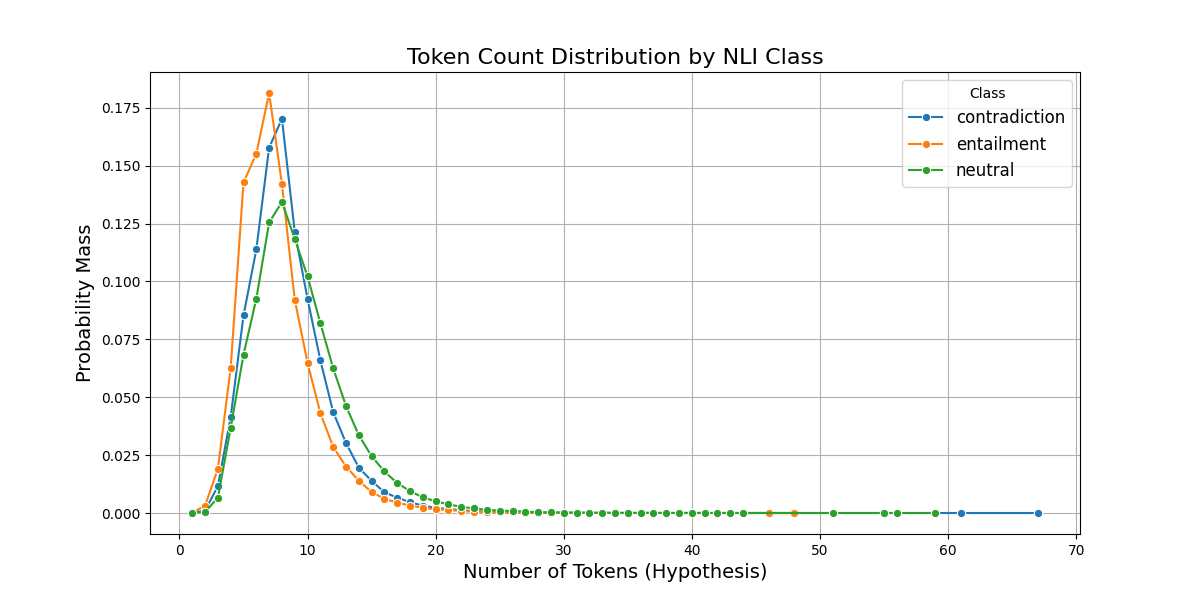
\includegraphics[width=1.0\linewidth]{Figure_tokenvsprobmass.png}
    \caption{Probability Mass Function of Hypothesis Length by Class, SNLI}
    \label{fig:ProbMassLength}
\end{figure}
Figure \ref{fig:ProbMassLength} shows the probability word mass of each class within the SNLI corpus. Note that the entailed class has the highest probability of less than 7 word tokens on average per hypothesis, while neutral has the widest distribution skewed towards the highest number of tokens of any of the classifications.
\subsection{Evaluation Metric Explanations}
Natural Language Inference tasks have inspired a number of standard datasets, each slightly different in intended task.  Stanford's NLI (SNLI) is the original dataset for NLI testing containing about 570k sentence pairs. It was built from Flickr30k image dataset that contained photo descriptions of the pictures.  The hypotheses were then human generated via crowd sourcing responses. The dataset is balanced between the three classes of entailment, neutral, and contradiction, although it does contain spelling  and other errors.  It was built to be a basis and starting point for NLI testing as described in \citealp{dataAug}.

MultiNLI (MNLI) expanded upon the SNLI dataset by including genres outside of the original set. It consists of about 433k sentence pairs across ten distinct genres of written and spoken text. MNLI is not a balanced dataset across genres. The dataset is also split into matched and unmatched sentence pairs. Matched indicates that the pairs came from the same genre, while unmatched indicates that they came from different genres.  This dataset was introduced in 2018 to expand upon the weaknesses of the SNLI dataset as described in  \citealp{williams2018broadcoveragechallengecorpussentence}.

There are more NLI datasets specific to clinical, cross-lingual, heuristic and more data that we will not be discussing as part of this paper.

Benchmark testing for language models generally revolves around the accuracy metric, which is fine unless the dataset is unbalanced. 

\begin{equation*}
\text{Accuracy} = \frac{\text{total correct}}{\text{total size of testset}}
\end{equation*}

In an unbalanced test set, this metric does not reflect enough information regarding the model's weaknesses between different classes. However, since SNLI is a balanced dataset, accuracy is a useful metric to include along with other investigations that illuminate a model's true weaknesses in language interpretation.

The F1 score is useful in unbalanced datasets or where we need to know the percent of false positives/false negatives. F1 score is the harmonic mean of the model's Precision and Recall scores. Precision is the accuracy of positive predictions, while Recall is how well the model can correctly identify positive predictions.
\begin{equation*}
\text{F1} = \frac{\text{2 * Precision * Recall }}{\text{Precision + Recall}}
\end{equation*}
\begin{equation*}
\text{Precision} = \frac{\text{Correctly predicted Positives}}{\text{True Positives+False Positives}}
\end{equation*}
\begin{equation*}
\text{Recall} = \frac{\text{Correct Positive Predictions}}{\text{True Positives + False negatives}}
\end{equation*}

In the case of NLI, this metric is useful in determining how effectively the model separates relevant information from irrelevant information.  In our testing, it was found that within the SNLI dataset this metric was extremely close to the accuracy, as expected due to the balanced nature of the dataset. When evaluating the contrast data set, there was a slightly larger differential from accuracy because the contrast set is not as balanced as the original.

Lastly, confidence scores are also extremely useful in identifying how much a model relies on data artifacts to make decisions. When a model mispredicts with high confidence, there is likely an identifiable pattern which can be discerned and around which one can focus training. Confidence is calculated as the probability of each class from the model output, with the probability of the true label returned as the model confidence for that prediction.
\begin{equation*}
\text{Confidence} = \frac{e^{\text{Model Logits}}}{\sum e^{\text{Model logits}}}
\end{equation*}

\section{Related Works}
Existing approaches to improving NLI tasks for models such as ELECTRA utilize some form of debiasing methods to remove spurious artifacts learned by a model.

Adversarial training is one debiasing method utilized to improve a model's language inference. These datasets are created specifically to challenge a model's heuristics as described in \citealp{adversarial1}, or to find universal triggers that always make the model predict incorrectly, as found in \citealp{wallace2021universaladversarialtriggersattacking}. One must be careful with how adversarial the perturbations are, lest it get too aggressive and reduce the model's ability to understand language.

Another option is to utilize Checklist for task agnostic testing of model behaviors. Checklist is a tool that helps fully test a model on multiple tasks, as defined by the user. In this case, it can be used to identify artifacts through controlled perturbing specific linguistic features, as described in \citealp{checklist}.

Contrast datasets are similar to adversarial training, but their intention is to more clearly identify the difficult pivot points between similar inputs. The intention here is to perturb the hypothesis in ways which illustrate where the model is having difficulty separating different classifications, possibly due to reliance on artifacts, as illustrated in  \citealp{localdecisionboundaries}.

\section{Model}
\subsection{Pre-trained Model}

We began with a pre-trained Electra Small Discriminator model from HuggingFace. For the NLI (Natural Language Inference) task, the ElectraForSequenceClassification head was selected as the fine tuning head.

ELECTRA small has a vocabulary size of ~30k, with an embedding size of 128, hidden size of 256 with 12 hidden layers, and 4 attention heads.  It is significantly smaller than the regular ELECTRA or other similar models. While this allows for faster and more accessible training, there is a small trade-off in its ability to understand more complex tasks or handle large datasets.

Initially ELECTRA small was fine-tune trained on the SNLI dataset for 3 epochs. At this point, the model was able to achieve 89\% accuracy on the evaluation set. 

Retraining the model on half the SNLI dataset for 5 epochs decreased the model accuracy to 88.6\%, indicating that the amount of the dataset used in training is at least as important as the number of epochs it is trained for.  

Evaluating the model predictions demonstrated some very high confidence mispredictions, largely skewing toward predicting neutral when the model was incorrect.

\subsection{Evaluation Trials}
In order to identify where the model was having difficulty discerning classification, we altered the code to save all incorrectly predicted premise/hypothesis pairs, including their gold label, model output prediction array, and predicted label to a file. A single line of which is illustrated in Table \ref{tab:SavedInfo1}.
\begin{table}[!ht]
    \centering
    \begin{tabularx}{0.45\textwidth}{ 
  | >{\raggedright\arraybackslash}X 
  | >{\raggedright\arraybackslash}X | }
    \hline
        Premise & Two men on bicycles competing in a race  \\
        \hline
        Hypothesis & Men are riding bicycles on the street. \\
        \hline
        Gold Label & 1 \\
        \hline
        Predicted Scores & 0.8896671, -0.29746633, -0.7488353\\
        \hline
        Predicted Label & 0\\
        \hline
    \end{tabularx}
    \caption{Information saved from Model Errors}
    \label{tab:SavedInfo1}
\end{table}

Given the understanding that there are data artifacts that rely on the length of the hypothesis to determine neutral classification, we evaluated the frequency of average number of tokens in the hypothesis across the mispredicted set. The results of this analysis on the dataset are found in Figure \ref{fig:EarlyTokenCount}.
\begin{figure}[h!]
    \centering
    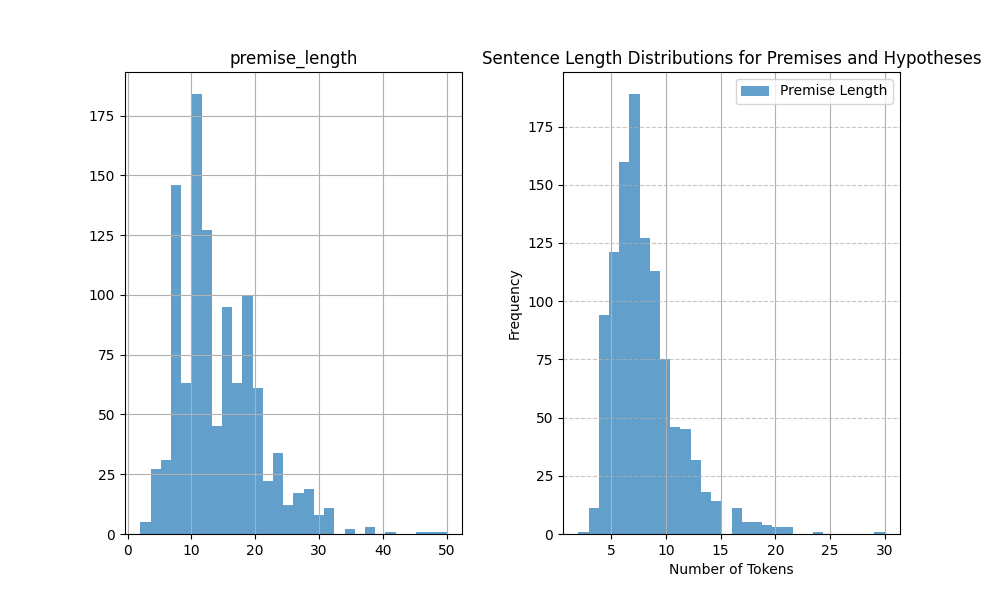
\includegraphics[width=0.85\linewidth]{FigurePremiseHypoWordCountFrequency.png}
    \caption{Frequency of Number of Word Tokens in Mispredictions after SNLI fine tune only}
    \label{fig:EarlyTokenCount}
\end{figure}
The SNLI dataset as a whole has the most number of premises in the 10-15 token range and hypothesis in the 5 to 10 word token range. The errors were not that different from this same pattern, being slightly above the token count on the premise, but in the same range for the hypothesis.

Next, we calculated the confidence for each error and included it in the output file as shown in Table \ref{tab:SavedInfo2}. Initially, the high confidence errors were used to hand build the contrast set. While this did make some changes to the model's decision structure, it was not the most effective subset to start with.  It made much more sense to start with the low confidence errors since those should be easier to perturb in the correct direction.
\begin{table}[!ht]
    \centering
    \begin{tabularx}{0.45\textwidth}{ 
  | >{\raggedright\arraybackslash}X 
  | >{\raggedright\arraybackslash}X | }
    \hline
        Premise & Two men on bicycles competing in a race  \\
        \hline
        Hypothesis & Men are riding bicycles on the street. \\
        \hline
        Gold Label & 1 \\
        \hline
        Predicted Scores & 0.8896671, -0.29746633, -0.7488353\\
        \hline
        Predicted Label & 0\\
        \hline
        confidence & 0.20348247\\
        \hline
    \end{tabularx}
    \caption{Information saved from Model Errors included Confidence Scores}
    \label{tab:SavedInfo2}
\end{table}
Visual inspection of the output file illuminated a noticeable volume of failures when the premise was a compound sentence and the hypothesis was clearly entailed by the first half and not the second. One such example is found in Table \ref{tab:1sthalfentailment}.
\begin{table}[h!]
    \centering
    \begin{tabularx}{0.45\textwidth} { 
  | >{\raggedright\arraybackslash}X 
  | >{\raggedright\arraybackslash}X | }
    \hline
        Premise & A group of people plays a game on the floor of a living room while a TV plays in the background.\\
        \hline
        Hypothesis & A group of people are sitting on the floor.\\
        \hline
    \end{tabularx}
    \caption{Example of long premise with early entailment}
    \label{tab:1sthalfentailment}
\end{table}
There were also examples where the hypothesis used the same adjectives and nouns as the premise, but not in the same way or attached to the same nouns. Where the model should have predicted contradiction, it predicted entailment likely from reliance on the words but not the meaning of the sentence. One such example is in Table \ref{tab:samewordswrongmeaning}.
\begin{table}[h!]
    \centering
    \begin{tabularx}{0.45\textwidth} { 
  | >{\raggedright\arraybackslash}X 
  | >{\raggedright\arraybackslash}X | }
    \hline
        Premise & A man in a blue shirt, khaki shorts, ball cap and white socks and loafers walking behind a group of people walking down a stone walkway with a water bottle in his left hand.\\
        \hline
        Hypothesis & A man in a blue shirt, khaki shorts, ball cap and blue socks and loafers walking behind a group of people walking down a stone walkway with a water bottle in his left hand.\\
        \hline
    \end{tabularx}
    \caption{Example of same words but different meanings}
    \label{tab:samewordswrongmeaning}
\end{table}
We also found a number of pairs that required true inference to predict correctly. A human would never have difficulty understanding that throwing any food item was a food fight, but the model did not understand that (i.e. "they were throwing tomatoes at each other" - "they were having a food fight").

Using these visual inspections and the confidence scores, along with filtering the data for specific groupings of errors (entailment as contradiction and vice versa, etc), a contrast dataset was hand built.  For each error, we included original premise/hypothesis then added two more hypotheses paired with the same premise. The additions were perturbed such that one did not alter the label, while the other altered it to the incorrectly predicted label. The intention was to bring the similar labels closer together and push the different labels further apart.  Examples can be found in the Contrast Sets section in Tables \ref{tab:Annot1} and \ref{tab:Annot2}.
 \section{Analysis of errors}
\subsection{Testing Procedure and Results}
After initial fine tune training, the model was evaluated against the SNLI and GLUE benchmarks. As a baseline, the accuracy and F1 scores of each were as follows in Table \ref{tab:basescores}.
\begin{table}[!ht]
    \centering
    \begin{tabularx}{0.45\textwidth} { 
  | >{\raggedright\arraybackslash}X 
  | >{\centering\arraybackslash}X
  | >{\raggedright\arraybackslash}X | }
    \hline
        Test set & Accuracy & F1 Score\\
        \hline
        SNLI & 89\% & 89\%\\
        \hline
        GLUE:MNLI & 71\% & 71\%\\
        \hline
    \end{tabularx}
    \caption{Baseline Accuracy and F1 Scores}
    \label{tab:basescores}
\end{table}

Counting the incorrect labels demonstrated a tendency toward neutral, with entailment and contradictory both lower than gold label standard totals.

The initial contrast data set was build with the high confidence errors. It contained about 50 sentence pairs, where the original was kept and a perturbed hypothesis was added which altered the label. This proved to be the incorrect path to start as the high confidence predictions are harder to move. After creating this set and performing an evaluation on the model, the accuracy significantly dropped, to about 44\%.  This is as expected given these were the pairs the model struggled with, and no new training had been done to improve performance.

Upon researching how confidence best interacted with contrast testing, we decided to focus on low confidence errors prior to further testing and adding data augmentation. Our contrast set now contained around 70 entries. This set was used for data augmentation training. The model was trained on this contrast set for 3 epochs, then evaluated again on the contrast and SNLI sets. The SNLI accuracy was lower, but the contrast accuracy increased significantly as found in Table \ref{tab:scores1}.

\begin{table}[h!]
    \centering
    \begin{tabularx}{0.45\textwidth} { 
  | >{\raggedright\arraybackslash}X 
  | >{\centering\arraybackslash}X
  | >{\raggedright\arraybackslash}X | }
    \hline
        Test set & Accuracy & F1 Score\\
        \hline
        SNLI & 78\% & 78\%\\
        \hline
        Contrast & 72.6\% & 72.5\%\\
        \hline
    \end{tabularx}
    \caption{After Data Augmentation Fine Tuning with Contrast set}
    \label{tab:scores1}
\end{table}
Fine tune training with just the small Contrast set was likely causing major shifts on the model weights, which influenced the drop in SNLI accuracy. To combat this, the model was given a refresh training on a small subset of the SNLI dataset to bring the weights back in line with the SNLI corpus. This yielded a high 89.8\% accuracy on the SNLI dataset.

After the SNLI refresh, the model was then again retrained on the Contrast dataset, but the learning rate was held constant to prevent the small dataset from making major changes to the model weights. Given the learning rate during training on the SNLI datset was on the order 1e-5, it was decided to set the learning rate to 1e-6 for the Contrast refresh. This yielded no degradation in the SNLI accuracy, but increased the Contrast set accuracy as shown in Table \ref{tab:scores2}.
\begin{table}[h!]
    \centering
    \begin{tabularx}{0.45\textwidth} { 
  | >{\raggedright\arraybackslash}X 
  | >{\centering\arraybackslash}X
  | >{\raggedright\arraybackslash}X | }
    \hline
        Test set & Accuracy & F1 Score\\
        \hline
        SNLI & 89.6\% & 89.5\%\\
        \hline
        Contrast & 77.4\% & 77.3\%\\
        \hline
    \end{tabularx}
    \caption{SNLI Refresh, Contrast Refresh with constant learning rate}
    \label{tab:scores2}
\end{table}

The final two additions to the contrast set focused on contradiction predicted as entailment and entailment predicted as contradiction. This expanded the Contrast set to about 560 sentence pairs. We again followed the pattern of evaluating on the contrast set, refreshing the model training on a subset of SNLI, refreshing with constant low learning rate on the Contrast set, and then evaluating on SNLI and Contrast datasets. Each time the evaluation on the Contrast set without any additional training was around 46-49\% prior to retraining and refresh.  After retrain and refresh there were small increases in the GLUE:MNLI test, but the SNLI was able to nearly fully recover and the Contrast evaluation increased significantly each training. Table \ref{tab:scores3} illustrates this behavior.
\begin{table}[h!]
    \centering
    \begin{tabularx}{0.45\textwidth} { 
  | >{\raggedright\arraybackslash}X 
  | >{\centering\arraybackslash}X
  | >{\raggedright\arraybackslash}X | }
    \hline
        Test set & Accuracy & F1 Score\\
        \hline
        SNLI & 89.44\% & 89.45\%\\
        \hline
        Contrast & 80.9\% & 80.8\%\\
        \hline
        Glue:MNLI & 69.0 & 69.0\\
        \hline
    \end{tabularx}
    \caption{Final SNLI Refresh, Contrast Refresh with constant learning rate}
    \label{tab:scores3}
\end{table}

\subsection{Contrast Sets}
Contrast Sets are best described as pairing a premise with multiple hypotheses which either pull similar classification pairs closer together, or push dissimilar classification pairs further apart in an attempt to clarify the decision boundary for the model as discussed in \citealp{sanwal2024evaluatinglargelanguagemodels}.

Mathematically using Cosine Similarity is the best way to determine classification similarity between hypotheses. This metric will evaluate to a number between 0 and 1, where the lower the number the more similar the sentences.  Given the size of the SNLI dataset, we decided to work with the model's errors and hand create a Contrast dataset with the same intention.

Attacking the high confidence errors first, we added in the original sentence pair and then one which was perturbed to generate a different label. An example can be found in Table \ref{tab:Annot1}.
\begin{table}[h!]
    \centering
    \begin{tabularx}{0.45\textwidth} { 
  | >{\raggedright\arraybackslash}X 
  | >{\raggedright\arraybackslash}X | }
    \hline
        Premise & A man in a green jersey and rollerskates stumbles as a man in a black jersey appears to collide with him.\\
        \hline
        Original Hypothesis & They both fall to the ground.\\
        \hline
        Hypothesis 1 & The man falls to the ground.\\
        \hline
    \end{tabularx}
    \caption{Example from Contrast Dataset: High Confidence Error}
    \label{tab:Annot1}
\end{table}

Next we added in low confidence errors where similar to before, the original pairing as included along with another which either attempted to clarify the same label, or pushed it further to get the model to recognize it as a different classification. An example can be found in Table \ref{tab:Annot2}.
\begin{table}[h!]
    \centering
    \begin{tabularx}{0.45\textwidth} { 
  | >{\raggedright\arraybackslash}X 
  | >{\raggedright\arraybackslash}X | }
    \hline
        Premise & Two Asian women talking and having drinks at a small round table.\\
        \hline
        Original Hypothesis & Two ladies are sitting at the bar.\\
        \hline
        Hypothesis 1 & Two ladies are sitting at the table.\\
        \hline
    \end{tabularx}
    \caption{Example from Contrast Dataset: Low Confidence Error}
    \label{tab:Annot2}
\end{table}

After these initial perturbations, the model errors were evaluated for the confidence level by classification. This resulted in an interesting graphic showing that while both Neutral and Contradiction tapered off as confidence increased, Entailment had a few jumps along the x-axis as shown in Figure \ref{fig:Confidence1}.

\begin{figure}[h!]
    \centering
    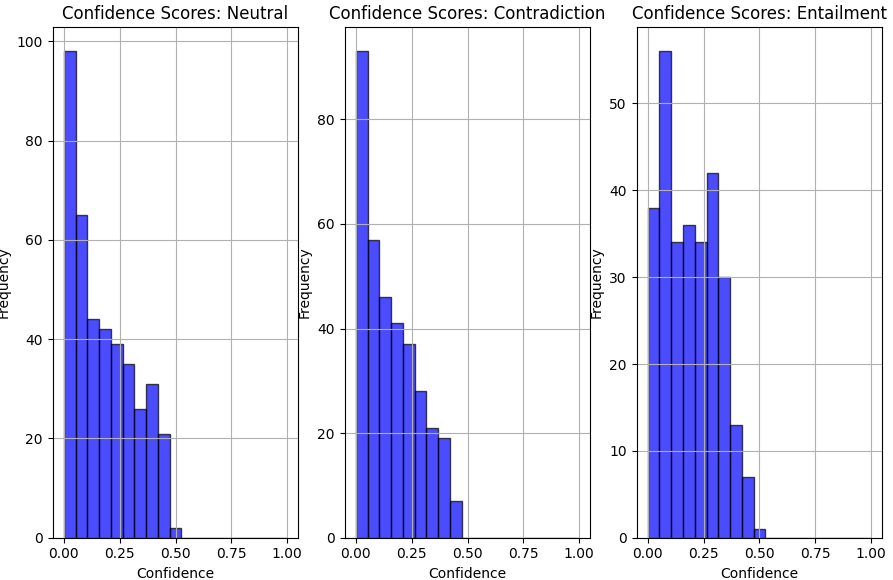
\includegraphics[width=0.75\linewidth]{FigureConfidenceByClass.png}
    \caption{Confidence by Classification}
    \label{fig:Confidence1}
\end{figure}

Even though the overall trend of the confidence level for Neutral and Contradiction were going in the ideal direction, there were still a few 50\% confidence ratings and significantly more errors in the higher percentages than would indicate the model was learning new connections with our current Contrast Dataset.  Checking the classification errors from the model against the gold label, it became obvious that the issue was between the two outer edge classes, Entailment and Contradiction. Counts of gold labels from errors and model predictions to illustrate this correlation are found in Table \ref{tab:ClassCount}.

\begin{table}[h!]
    \centering
    \begin{tabularx}{0.45\textwidth}{
  | >{\raggedright\arraybackslash}X 
  | >{\centering\arraybackslash}X
  | >{\raggedright\arraybackslash}X | }
    \hline
        & Gold Label & Prediction \\
        \hline
        Neutral & 462 & 461 \\
        \hline
        Entailment & 334 & 270 \\
        \hline
        Contradiction & 263 & 328 \\
        \hline
    \end{tabularx}
    \caption{Class Number: Gold vs Model}
    \label{tab:ClassCount}
\end{table}

Given this new information, additions to the Contrast set were created from filtered errors where the model predicted either Entailment or Contradiction, completely opposite the gold label. An example is found in Table \ref{tab:AnnotationOfContrastSet}.
\begin{table}[!ht]
    \centering
    \begin{tabularx}{0.5\textwidth} { 
  | >{\raggedright\arraybackslash}X 
  | >{\raggedright\arraybackslash}X | }
    \hline
        Premise & A brown dog with a blue muzzle is running on green grass.\\
        \hline
        Original Hypothesis & A dog is wearing a green muzzle on blue grass.\\
        \hline
        Hypothesis 1 & A dog is wearing a green grass on blue muzzle.\\
        \hline
        Hypothesis 2 & A dog is running a green grass in blue muzzle.\\
        \hline
    \end{tabularx}
    \caption{Example from Contrast Dataset}
    \label{tab:AnnotationOfContrastSet}
\end{table}

Upon the training refresh and evaluation with these additions, while the overall accuracy did not increase, the contrast accuracy and the GLUE:MNLI benchmark did increase. There was a marked change in the calculated confidence of the model. Overall the model became much less confident on the errors as show in Figure \ref{fig:Confidence3}.
\begin{figure}[h!]
    \centering
    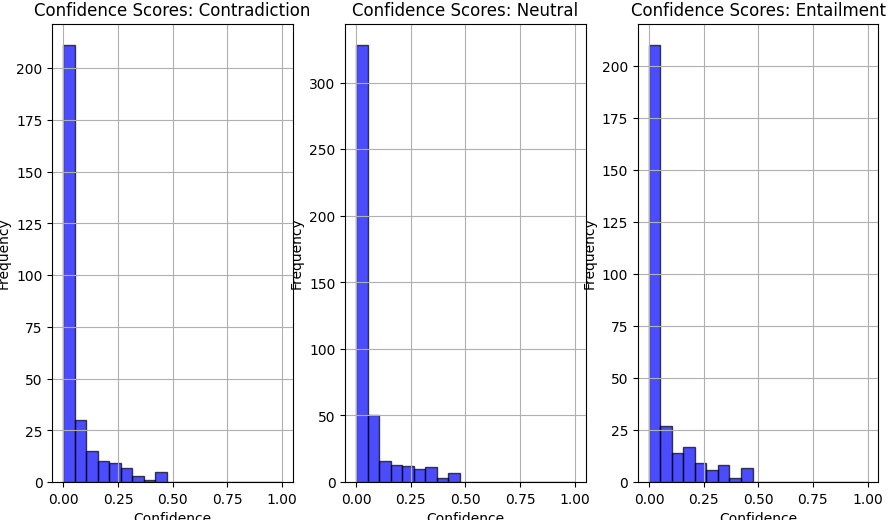
\includegraphics[width=0.85\linewidth]{Figure_confByClass3.png}
    \caption{Confidence per Class, Expanded Contrast Set}
    \label{fig:Confidence3}
\end{figure}
The significant drop in confidence values indicated the model is breaking from the artifacts it learned initially and moving toward more true inference of more complex language. With a more complete Contrast Set we have no doubt the model would have increased overall accuracy and performed significantly better in a real world language test bed.

\section{Conclusion}
The ELECTRA small model, pre-trained as a Replacement Token Detection model, and fine tuned on the SNLI dataset for Sentence Classification is fairly accurate in the test bed, but does not demonstrate such success in a real world test environment. The model clearly learned data artifacts that allowed it to classify sentence pairs. It sometimes was clearly not considering the premise at all in classification. Other times it classified by seeing consistent words in both the premise and hypothesis even though they were in a different order and altered the meaning of the sentence.
Performing evaluation on the model errors with known Data Artifacts, and including Confidence scores to help identify where the model was most able to be perturbed in the correct direction, lead to a Contrast Dataset which was able to decrease the model's reliance on said artifacts without degrading accuracy on the original test set.
We believe that with more work utilizing Cosine Similarity to create a complete Contrast Dataset, and performing additional fine tuning on the parameters for the model such as learning rate, training epochs, etc, ELECTRA small could be improved to increased performance in accuracy on the SNLI evaluation, Glue:MNLI, and in a real world test.
\bibliographystyle{apalike}
\bibliography{references}

\end{document}